\documentclass[a4paper]{article}

%% Language and font encodings
\usepackage[english]{babel}
\usepackage{amsthm, amsfonts}
\usepackage[utf8x]{inputenc}
\usepackage[T1]{fontenc}
\usepackage{listings}
\usepackage{algpseudocode, algorithm}
\usepackage{mathtools}
\usepackage{enumerate}
\usepackage{tabu}
\usepackage{xcolor}
\usepackage{tikz, tikz-qtree}
\usepackage{graphviz}
\usepackage{subfig}
\usepackage{blindtext}

%% Sets page size and margins
\usepackage[a4paper,top=3cm,bottom=2cm,left=3cm,right=3cm,marginparwidth=1.75cm]{geometry}

%% Useful packages
\usepackage{amsmath}
\usepackage{graphicx}
\usepackage[colorinlistoftodos]{todonotes}
\usepackage[colorlinks=true, allcolors=blue]{hyperref}

\newenvironment{solution}{\begin{proof}[\textnormal{\textbf{Solution}}]}{\end{proof}}
\newenvironment{exercise}[1]{\begin{proof}[\textnormal{\textbf{Exercise #1:}}]\phantom{\qedhere}}{\end{proof}}
\newenvironment{lemma}{\begin{proof}[\textnormal{\textbf{Lemma}}]\phantom{\qedhere}}{\end{proof}}

\renewcommand\thesubfigure{\arabic{subfigure}}

\begin{document}
\begin{titlepage}\pagenumbering{gobble}
	\centering
	{\scshape\LARGE University of Houston\par}
	\vspace{1cm}
	{\scshape\Large Geometric Transformations of Images \par}
	\vspace{1.5cm}
	{\huge\bfseries COSC 4393 \par}
	{\huge\bfseries Digital Image Processing\par}
	\vspace{0.5cm}
	{\large\bfseries Pranav Mantini\par}
	\vspace{1cm}
	{\Large\itshape \begin{tabular}{|c|}\hline 
	                   \textcolor{blue}{\textbf{Wednesday}} \\\hline 
	                   Khalid Hourani\\\hline
	                   Conrad Parker\\\hline
	                   Morris Smith\\\hline
	                   Raymond Sutrisno\\\hline
	                   Jackson Murrell\\\hline
	                   Christian Wilson\\\hline
	                   Willard Boss\\\hline
	               \end{tabular}\par}
	\vspace{0.5cm}
	{\large \par} %date
	\vfill
% Bottom of the page
\end{titlepage}

\tableofcontents
\newpage\pagenumbering{arabic}

\section{Introduction}

A Geometric Transformation is any function \[f:\mathbb{R}^m\to\mathbb{R}^n\] In the case of image processing, we are concerned with functions from $\mathbb{R}^2$ to $\mathbb{R}^2$.

\href{https://github.com/TetroVolt/DIP-Project}{Our application} allows the user to apply various geometric transformations to images. This report describes these transformations and details some observations made during development and the ways these transformations can be used to determine properties of an image. 

All images in this report are transformations applied to the following image of Lenna.

\begin{figure}[H]
    \centering
    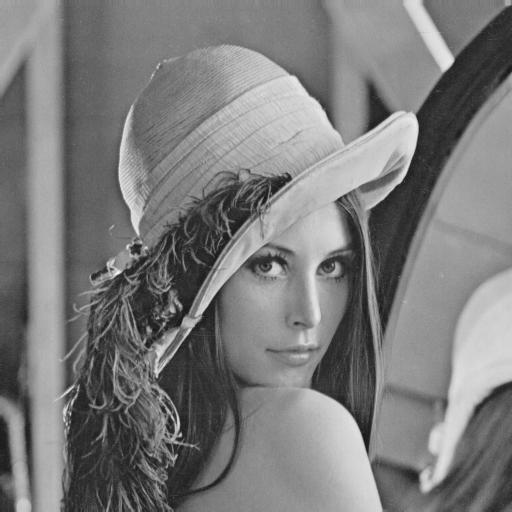
\includegraphics[scale=0.5]{images/lenna-grey.jpg}
    \caption{Lenna}
    \label{fig:lenna-original}
\end{figure}

\section{Geometric Transformations}
\subsection{Nearest Neighbor} \label{subsec:nearest-neighbor}

The \textbf{Nearest Neighbor Interpolation} takes an image $I_{M\times N}$ and new image dimensions $M'\times N'$ and resizes the image. Our \textit{transformed image} $I'_{M'\times N'}$ is obtained by applying the following transformation:

\[I'(x, y)=I\left(\left[\frac{x}{r_x}\right], \left[\frac{y}{r_y}\right]\right)\]

where $[x]$ denotes the nearest integer to $x$ and

\begin{align*} r_x &= \frac{M'}{M}\\
               r_y &= \frac{N'}{N}
\end{align*} are the \textit{scale factors}. In other words, we divide the values of $x$ and $y$ by their respective scale factors and look for the closest pixel in the original image, then assign the intensity value of that pixel to our transformed image. 

\begin{figure}[H]
    \centering
    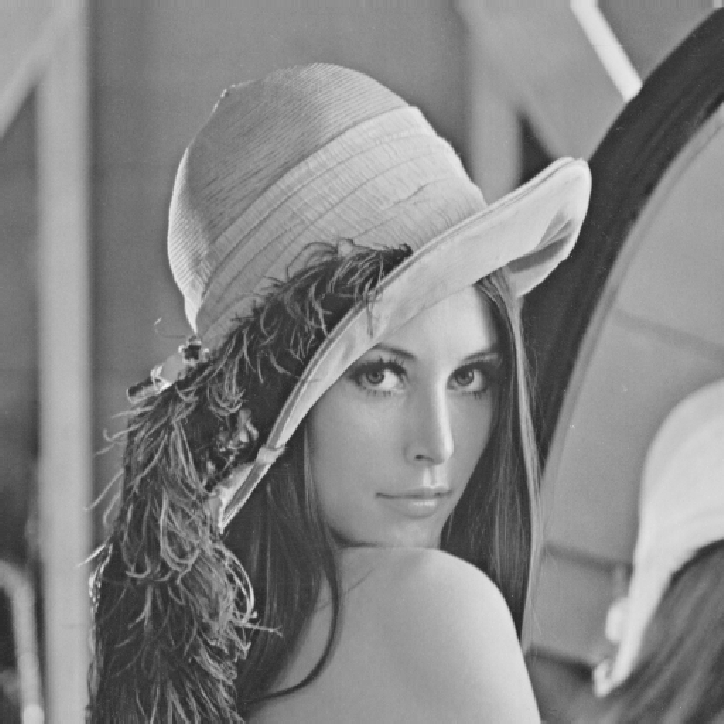
\includegraphics[scale=0.5]{images/lenna-nearest-neighbor.png}
    \caption{Nearest Neighbor Interpolation with scale $(\sqrt{2}, \sqrt{2})$}
    \label{fig:lenna-nearest-neighbor}
\end{figure}
\subsection{Bilinear} \label{subsec:bilinear}

\textbf{Bilinear Interpolation} resizes an image in the same vein as Nearest Neighbor, but applies linear interpolation three times. Specifically, if we have points $(x_0, y_0)$ and $(x_1, y_1)$, we perform linear interpolation at a point $x$ between $x_0$ and $x_1$:

\[y = y_0+(x-x_0)\frac{y_1-y_0}{x_1-x_0}\]

to determine the value of $y$. As a matter of convention, let $y=i(x,x_0, y_0, x_1, y_1)$ denote the linear interpolation at $x$ on points $(x_0, y_0)$ and $(x_1, y_1)$. Our Bilinear Interpolation is obtained with the following transformation

\[I'(x, y) = i\left(\frac{y}{r_y}, Y_0, p_0, Y_1, p_1\right)\]

where

\begin{align*}
    p_0 &= i\left(\frac{x}{r_x}, X_0, I(X_0, Y_0), X_1, I(X_1, Y_0)\right)\\
    p_1 &= i\left(\frac{x}{r_x}, X_0, I(X_0, Y_1), X_1, I(X_1, Y_1)\right)
\end{align*}

and

\begin{align*}
    X_0&=\left\lfloor\frac{x}{r_x}\right\rfloor\\
    X_1&=\left\lceil\frac{x}{r_x}\right\rceil\\
    Y_0&=\left\lfloor\frac{y}{r_y}\right\rfloor\\
    Y_1&=\left\lceil\frac{y}{r_y}\right\rceil\\
\end{align*}

In other words, we interpolate twice on the $x$-values, then a third time on the $y$-value. It is straightforward to show that the result is the same after interpolating twice on the $y$-values, then a third time on the $x$-value.

\begin{figure}[H]
    \centering
    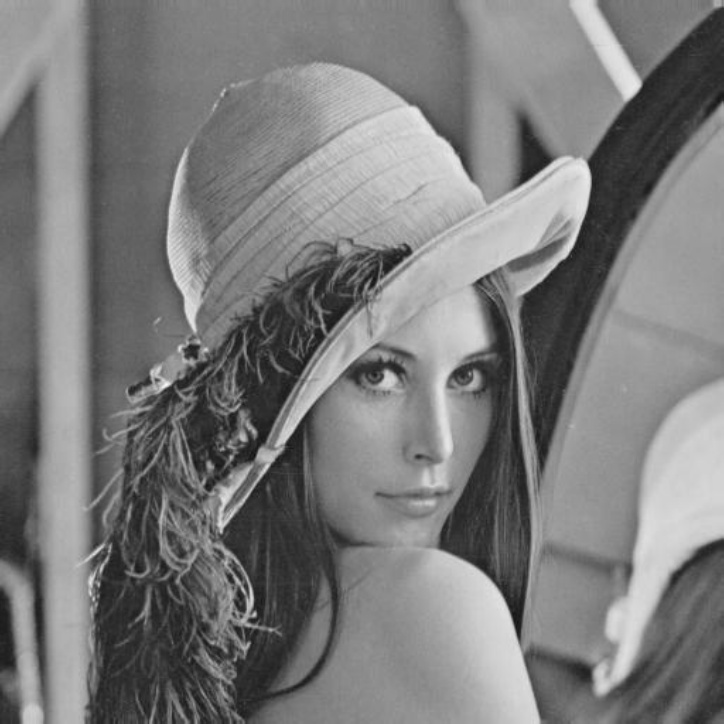
\includegraphics[scale=0.5]{images/lenna-bilinear.jpg}
    \caption{Bilinear Interpolation with scale $(\sqrt{2}, \sqrt{2})$}
    \label{fig:lenna-bilinear}
\end{figure}
\subsection{Bicubic} \label{subsec:bicubic}

A \textbf{Bicubic} interpolation interpolates from the nearest sixteen source points by performing five cubic interpolations. We use a Lagrange Polynomial on four points to determine a cubic function. That is, given $n+1$ points $(x_0,y_0), (x_1,y_1),\hdots, (x_n, y_n)$, there is a unique degree $n$ polynomial which exactly fits those $n+1$ points

\[P(x)=\sum_{i=0}^ny_i\ell_i(x)\]

where 

\[\ell_i(x)=\prod_{\substack{j=0\\j\neq i}}^n\frac{x-x_j}{x_i-x_j}\]

That $P(x_i)=y_i$ is straightfoward to show: for $j\neq i$, \[\ell_j(x_i)=0\] On the other hand, \begin{align*}\ell_i(x_i)&=\prod_{\substack{j=0\\j\neq i}}^n\frac{x_i-x_j}{x_i-x_j}\\&=1\end{align*} Thus, \begin{align*}P(x_i)&=\sum_{j=0}^ny_j\ell_j(x_i)\\&=\sum_{\substack{j=0\\j\neq i}}^ny_j\ell_j(x_i)+y_i\ell_i(x_i)\\&=0+y_i\cdot1\\&=y_i\end{align*}

To establish uniqueness, we show that if $q(x)$ is another degree-$n$ interpolating polynomial on these $n+1$ points, then $r(x)=p(x)-q(x)=0$. At each $x_i$, we have that $r(x_i)=0$, hence $r$ has $n+1$ roots and can be factored

\[r(x)=a(x-x_0)(x-x_1)\cdots(x-x_n)\]

However, $r$ must be of degree $n$, yet the expansion of the above expression results in a degree-$(n+1)$ polynomial $r$. This forces $a=0$. Thus, $r(x)=0$ and $p(x)=q(x)$. 

To interpolate at point $(x, y)$, we find sixteen nearby source points and interpolate horizontally four times. We then interpolate one final time, vertically. 
\begin{figure}[H]
    \centering
    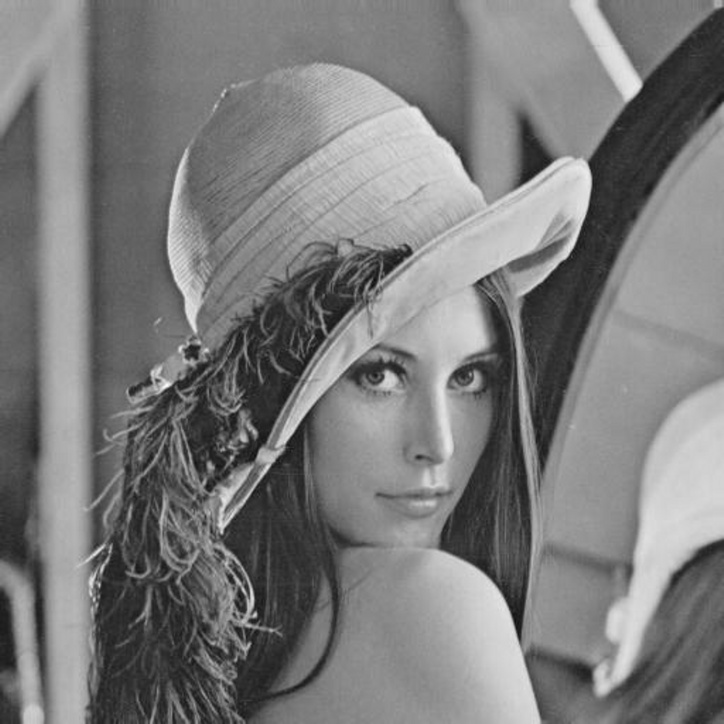
\includegraphics[scale=0.5]{images/lenna-bicubic.jpg}
    \caption{Bicubic Interpolation with scale $(\sqrt{2}, \sqrt{2})$}
    \label{fig:bicubic}
\end{figure}
\subsection{Lanczos} \label{subsec:lanczos4}

The Lanczos interpolation of order $n$ is a function:

\[L(x, n) =   \begin{cases}
    \text{sinc}(x)\cdot\text{sinc}(\frac{x}{n}) & \text{for } |x|\leq n \\
    0 & \text{otherwise}
  \end{cases}\]

where 

\[\text{sinc}(x) =   \begin{cases}
    1 & \text{for } x=0 \\
    \frac{\sin{\pi x}}{\pi x} & \text{otherwise}
  \end{cases}\]
  
To interpolate a two-dimensional image $I$, we define a filter weight $w$:

\[w = \sum_{i=-n+1}^n\sum_{j=-n+1}^n L(i-x + \lfloor x\rfloor, n)\cdot L(j - y + \lfloor y\rfloor, n)\]

and determine the intensity value of a pixel at $(x, y)$ with 

\[I'(x,y)=\frac{1}{w}\sum_{i=-n+1}^n\sum_{j=-n+1}^n I(\lfloor x\rfloor + i, \lfloor y\rfloor + j)\cdot L(i-x + \lfloor x\rfloor, n)\cdot L(j-y + \lfloor y\rfloor, n)\]

\begin{figure}[H]
    \centering
    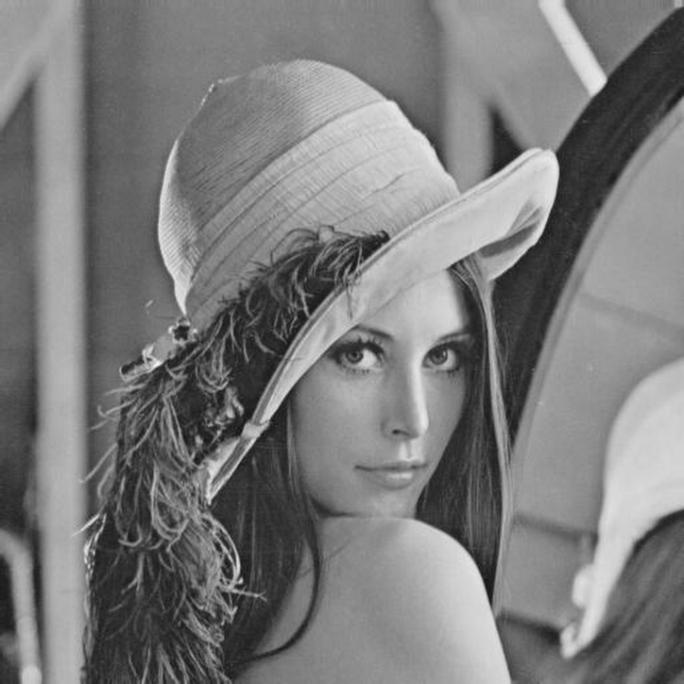
\includegraphics[scale=0.5]{images/lenna-lanczos4.jpg}
    \caption{Lanczos Interpolation of order 4 with scale $(\sqrt{2}, \sqrt{2})$}
    \label{fig:lenna-lanczos4}
\end{figure}
\section{Affine Transformations}
\subsection{Affine Warp}

An \textbf{Affine Transformation} is a transformation that preserves colinearity and ratios of distances: if $f$ is an affine transform and $p$ and $q$ are colinear points, then $f(p)$ and $f(q)$ are colinear and for any $w$ in the line containing $p$ and $q$, \[\frac{d(p, w)}{d(p,q)}=\frac{d(f(p), f(w))}{d(f(p),f(q))}\] Given an image $I_{M\times N}$ and a $2\times3$ matrix $A$, we transform the image $I$ as follows:

\[I'(x, y) = I\left(A\begin{bmatrix}x \\ y \\ 1\end{bmatrix}\right)\]

In particular, our choice of $A$ determines the type of affine transformation. 
\subsection{Rotation}

We rotate an image $I_{M\times N}$ around center $C=(c_x, c_y)$ by angle $\theta$ with scale factor $r$ by applying the affine transformation using \[A=\begin{bmatrix}\alpha & \beta & x_t\\-\beta & \alpha & y_t\end{bmatrix}\] where 
\begin{align*}\alpha &= r\cos\theta\\
               \beta &= r\sin\theta\\
               x_t &= C\begin{bmatrix}1 - \alpha & -\beta\end{bmatrix}\\
               y_t &= C\begin{bmatrix}\beta & 1 - \alpha\end{bmatrix}
\end{align*}

\begin{figure}[H]
    \centering
    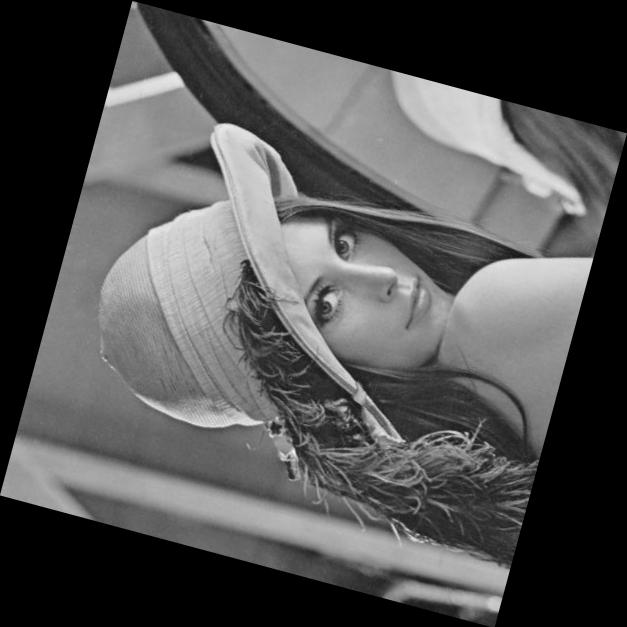
\includegraphics[scale=0.5]{images/lenna-rotation.jpg}
    \caption{Rotation of $75^{\circ}$}
    \label{fig:lenna-rotation}
\end{figure}
\subsection{Shear}

\subsection{Fisheye} \label{subsec:fisheye}

The basic principle behind a Fisheye transformation is in the creation of a map. The goal is to create a map for every pixel in the original image and then approximate the value of that pixel to a new location determined by the map. 

With a Fisheye transformation we are usually taking a square or rectangular image and converting it to a circle, with varying degrees of distortion as you approach the edge of the circle. 

Begin with an image $I_{M\times N}$. Initially, we create an array $A_{M\times N}$ with $A_{i,j}=(i,j)$. We then resize this array to be a $2\times\frac{M\cdot N}{2}$ matrix. Now, each row represents an $(x,y)$ pair. We compute the median value of this array and use it to determine the distance each $(x,y)$ pair is from the center of the image. We then have an $x$ distance and a $y$ distance for each pair. We use these as the two lines of a right triangle opposite the hypotenuse. We then apply the Pythagorean Theorem to determine the length of the radius, which is the hypotenuse of the triangle. 

After that, it is just a matter of reducing that radius and curving the edges. This is done by reducing the radii in half and normalizing for the total variance in distances. We then collapse them and use a formula that as pixels get closer to the edge they stack closer together. After that a simple use of geometric formulas produces the new $x$ and $y$ distances from the center of the image using our new radii, and we have our map. 

This map is applied with nearest neighbor interpolation to determine which pixel is taken from the original image and used in the new image.

\begin{figure}[H]
    \centering
    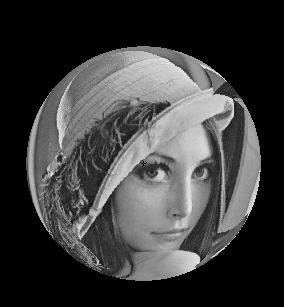
\includegraphics[scale=0.5]{images/fisheye.png}
    \caption{Fish Eye Transformation}
    \label{fig:lenna-fish-eye}
\end{figure}
\subsection{Perspective Warp} \label{subsec:perspective_warp}

\begin{figure}[H]
    \centering
    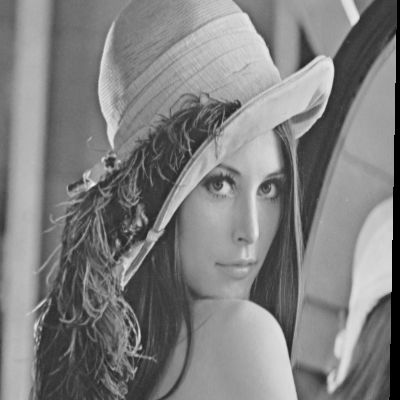
\includegraphics[scale=0.5]{images/lenna-perspective-warp.png}
    \caption{Perspective Warp}
    \label{fig:lenna-perspective-warp}
\end{figure}
\section{Observations}
\subsection{Interpolation Methods}
There are several, distinct differences between the various interpolation methods implemented in our project.

The most basic interpolation method is \textit{Nearest Neighbor} which was discussed in detail in \autoref{subsec:nearest-neighbor}.
While it has very good performance, it tends to result in a loss of detail. It is able to result in sharper images however, as it does not calculate missing values, and uses the values from the original image, so this sharpness becomes a trade-off for blocky artifcating.

To contrast this, we have \textit{Bilinear} (\autoref{subsec:bilinear}) which attempts to ``fill in the gaps'' of missing data. As such, it is more computationally expensive as it involves a calculation on three points for each pixel. This results in finer detail, but can also result in blurrier images. It also tends to leave cross artifacts as opposed to the blocky artifacts from \textit{Nearest Neighbor}, though these are much less noticeable.

\textit{Bicubic} interpolation (\autoref{subsec:bicubic}) requires significant computational processing, so it is not always feasible to use for very large images. However, the quality of the images that result is noticeable, especially at high zooms. It does not have the same artifcating issue that \textit{Bilinear} has, and while still a bit blurry, is much smoother overall.

The various artifacting elements mentioned here are most noticeable along edges.  Flat/smooth surfaces, solid colors or repeating textures, like a wall, the sky, or a persons cheek won't have as noticeable of an artifacting effect because the ``guess'' that the interpolation makes is relatively close to what would actually be there if we had zoomed in.  The blue color of the sky won't change as often or as drastically as the edge of a person's smile, so we won't notice any missing values as easily.

\begin{figure}[H]
    \centering
    \subfloat[Nearest Neighbor]{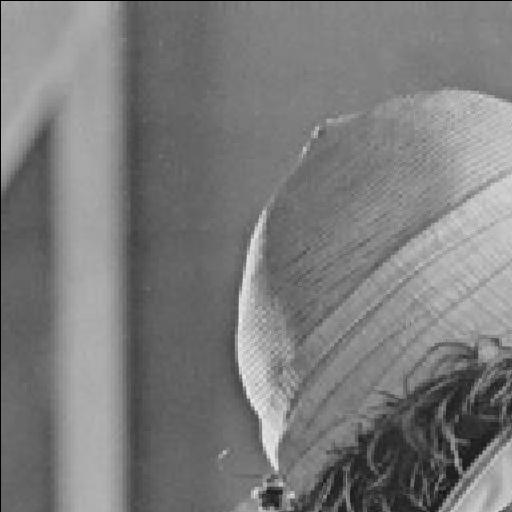
\includegraphics[width=0.4\textwidth]{images/lenna-nearest-neighbor-zoom.jpg}}
    \qquad
    \subfloat[Bilinear]{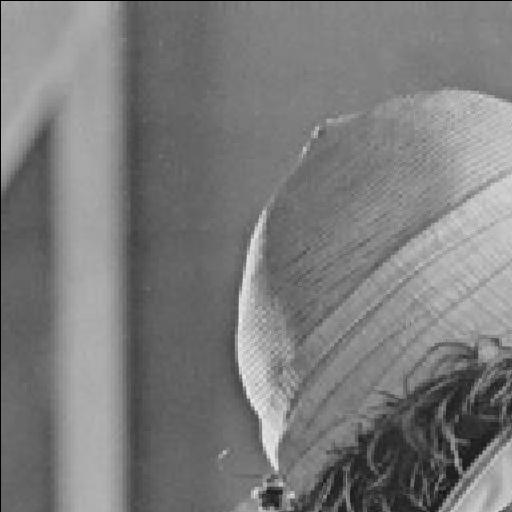
\includegraphics[width=0.4\textwidth]{images/lenna-bilinear-zoom.jpg}}
    \qquad\\
    \subfloat[Bicubic]{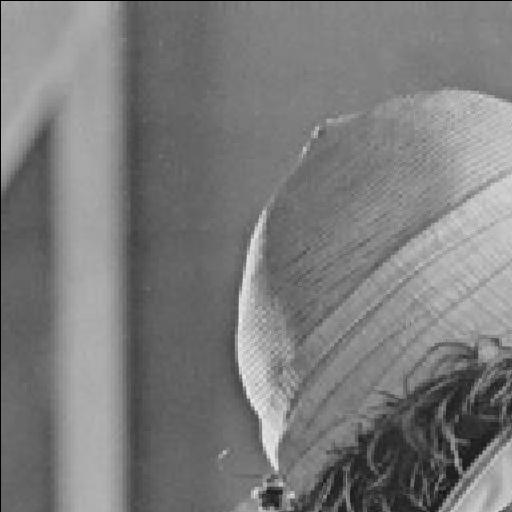
\includegraphics[width=0.4\textwidth]{images/lenna-bicubic-zoom.jpg}}
    \qquad
    \subfloat[Lanczos]{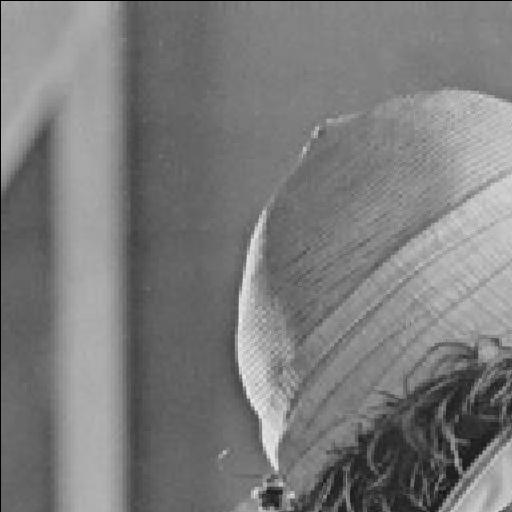
\includegraphics[width=0.4\textwidth]{images/lenna-lanczos4-zoom.jpg}}
    \caption{Side-by-Side comparison of zoomed-in interpolated images with scale $(2, 2)$}
    \label{fig:comparison}
\end{figure}
\subsection{Perspective Warp} \label{subsec:perspective_observations}
Perspective warping or transforms, as mentioned in \autoref{subsec:perspective_warp}, can change the desired area of an image to be the focal point, as if you were looking at it straight on.  This is a very useful feature in image recognition as it allows you to select a feature to look at without distortions from being at an angle, or far away.  For instance, we could do a perspective to make it appear as if the camera is looking down somewhat.


\end{document}